%%%%%%%%%%%%%%%%%%%%%%%%%%%%%%%%%%%%%%%%%%%%%%%%%%%%%%%%%%%%%%%%%%%%%%%%
% Plantilla TFG/TFM
% Universidad de A Coruña. Facultad de Informática
% Realizado por: Welton Vieira dos Santos
% Modificado: Welton Vieira dos Santos
% Contacto: welton.dossantos@udc.es
%%%%%%%%%%%%%%%%%%%%%%%%%%%%%%%%%%%%%%%%%%%%%%%%%%%%%%%%%%%%%%%%%%%%%%%%


\chapter{Modelo de conocimiento}
\newpage
\section{Fase de identificación}
\subsection{Tareas del formulario OM-3}
Las tareas elegidas para este modelo conceptual han sido las tareas 2, 3 y 4 del OM-3 (Tabla \ref{tab:IdentificacionOM3}), que corresponden con \textbf{Generar lista de entregas según ruta asignada}, \textbf{Determinar los recursos disponibles por la sucursal MRW para entregar según ruta} y \textbf{Revisión y validación de la distribución de la paquetería}.

\begin{table}[H]
  \centering
  \resizebox{15,0cm}{!}{
    \begin{tabular}{|c|c|c|c|c|c|c|}
      \hline
      \multicolumn{3}{|c}{\textbf{Modelo de Organización}} & \multicolumn{4}{|c|}{\textbf{Formulario OM-3: Descomposición de los Procesos}}\\
      \hline \hline
      
      \multicolumn{1}{|p{1.0cm}|}{\centering \textsc{N\textordmasculine}} &\multicolumn{1}{|p{3.0cm}|}{\centering \textsc{Tarea}} & \multicolumn{1}{|p{3.0cm}|}{\centering \textsc{Realiza\-da por}} & \multicolumn{1}{|p{3.0cm}|}{\centering \textsc{¿Dónde?}} & \multicolumn{1}{|p{3.0cm}|}{\centering \textsc{Recursos de Conocimiento}} & \multicolumn{1}{|p{3.0cm}|}{\centering \textsc {¿In\-ten\-si\-va en Conocimiento?}} & \multicolumn{1}{|p{3.0cm}|}{\centering \textsc{Im\-por\-tan\-cia}} \\
      \hline

      3 & \multicolumn{1}{|p{3.0cm}|}{\centering Determinar los recursos disponibles por la sucursal MRW para entregar según ruta} & \multicolumn{1}{|p{3.0cm}|}{\centering Equipo Directivo, Repartidor experimentado} & \multicolumn{1}{|p{3.0cm}|}{\centering En la nave de la sucursal de MRW} & \multicolumn{1}{|p{3.0cm}|}{\centering Experiencia en distribución de recursos. Utilizar teoria de programación dinámica} & Sí (elevado) & Máxima \\
      \hline
    \end{tabular}
  }
	\caption{\label{tab:IdentificacionOM3}Tarea elegida para el modelo de conocimiento}
\end{table}

\subsection{Glosario de términos}
\begin{itemize}
	\item \textbf{Paquete:} Envoltorio que contiene cualquier tipo de objeto. Se utiliza tambien para indicar los sobres.
	\item \textbf{Ruta:} Camino conformado por un número determinado de nodos (paradas) con un principio y un final que se cubre con un vehículo de reparto.  
	\item \textbf{Destinatario:} Persona o entidad que recibe un paquete.
	\item \textbf{Remitente:} Persona o entidad que envía o remite a otra persona un paquete.
	\item \textbf{Incidencia:} Circunstancia que impide una entrega.
	\item \textbf{Plataforma:} Local de asignación de envíos.
	\item \textbf{Envío:} Agrupación para uno o mas paquetes de un mismo destinatario.
	\item \textbf{Recogida:} Forma en la que el destinatario recoge el paquete de un remitente.
\end{itemize}

\subsection{Descripción de escenarios}
\begin{enumerate}
	\item  \textbf{Escenario de reducción de riesgo de una orden de compra (Buy):} En la situación que se muestra en la Figura \ref{fig:Situacion1}, donde el inversor había ejecutado una orden de compra en el precio \textbf{1.18767} y ha estipulado su gestión de riesgo para el precio \textbf{1.18664} y como se observa en el gráfico de la figura comentada anteriormente, el precio esta a favor del inversor y en esa ocasión el inversor tiene que reducir el riesgo inicial de la inversión al precio \textbf{1.19516} como se muestra en la Figura \ref{fig:Situacion12}.	
	\item  \textbf{Escenario de gestión de ganancia en una orden de compra (Buy)}: En la situación que se muestra en la Figura \ref{fig:Situacion2}, donde el inversor había ejecutado una orden de compra en el precio \textbf{1.18767} y ha estipulado su gestión de riesgo para el precio \textbf{1.18664} y como se observa en el gráfico de la figura comentada anteriormente, el precio esta a favor del inversor y el mismo decide cerrar esa operativa a precio del mercado, que en ese caso es de \textbf{1.19665}.	
\end{enumerate}

\section{Fase de especificación}
\subsection{Justificación de la selección de la metodología}
Para este proyecto hemos decidido utilizar la metodología ``middle-out'' con la selección de la plantilla de diseño, ya que esa plantilla nos permite diseñar la disposición de la paquetería en los vehículos de carga. 

\subsection{Plantilla anotada}

La plantilla que mas se adapta a nuestro problema es la de diseño, como se muestra en la Figura \ref{fig:PlantillaDiseno}. Con una pequeña modificación que se muestras en la Figuras \ref{fig:PlantillaDiagnosticoModificada}.

\begin{figure}[H]
  \centering
  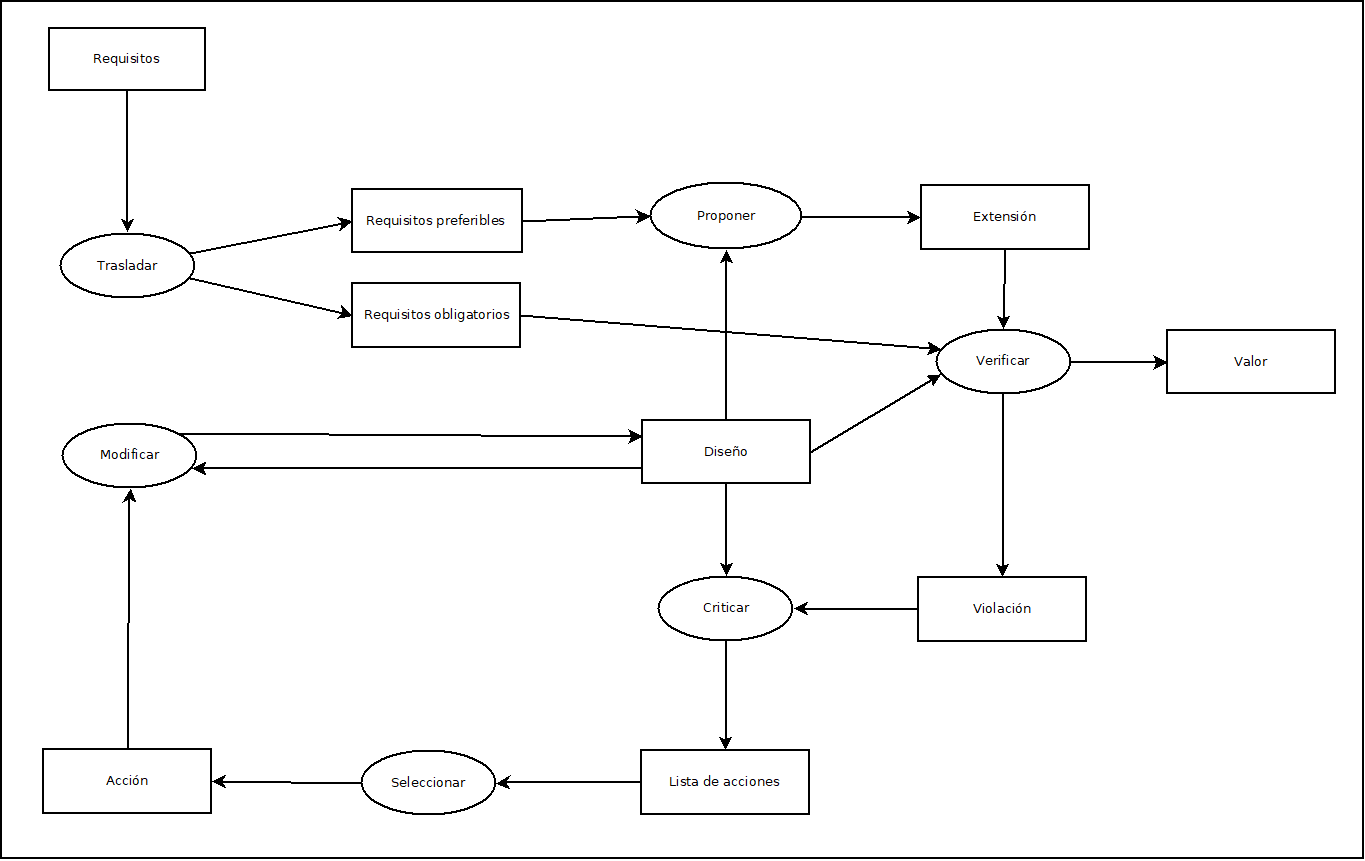
\includegraphics[scale=0.30]{imaxes/PlantillaConfiguracion.png}
  \caption{\label{fig:PlantillaDiseno}Ejemplo de la plantilla elegida}
\end{figure}

\begin{figure}[H]
  \centering
  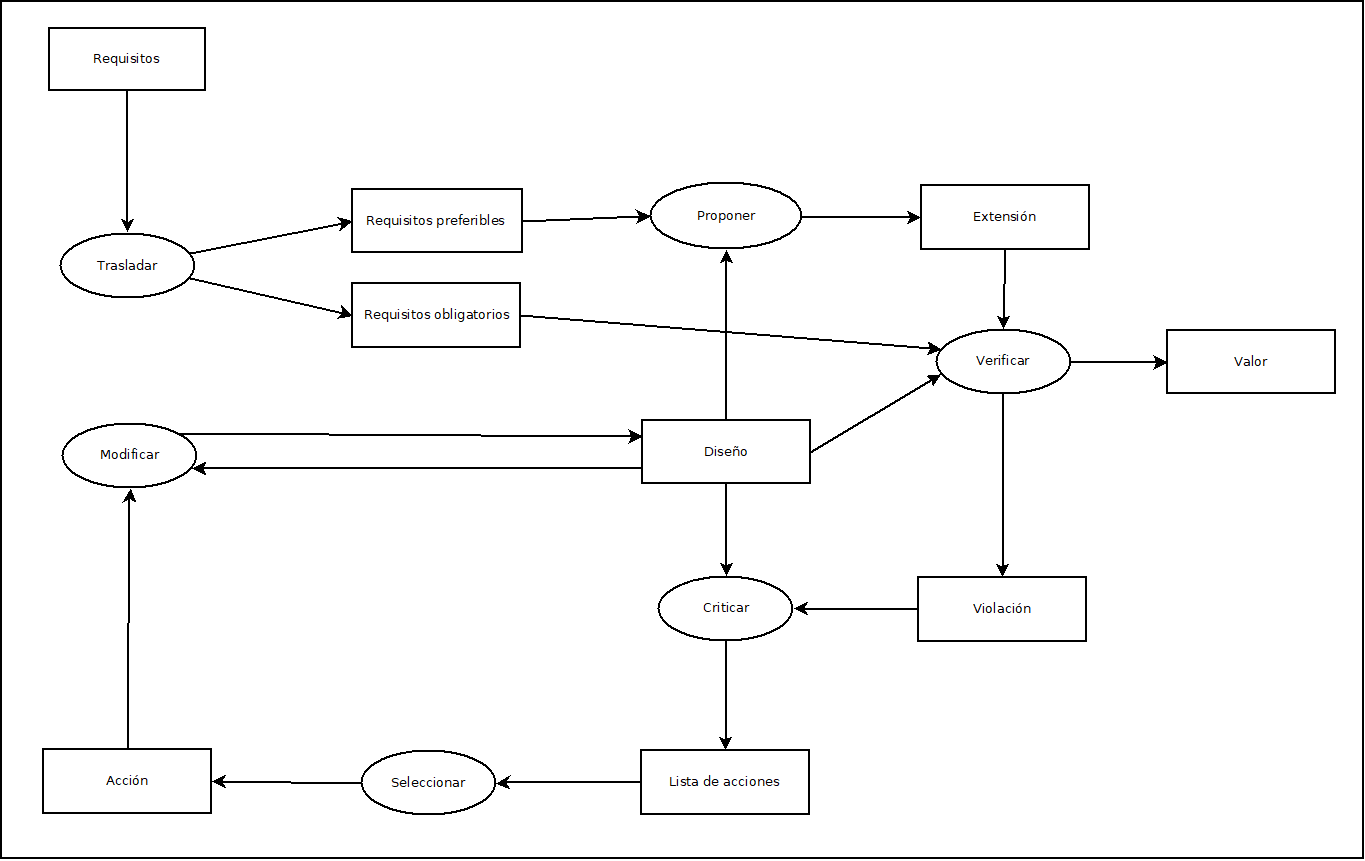
\includegraphics[scale=0.30]{imaxes/PlantillaConfiguracion.png}
  \caption{\label{fig:PlantillaDiagnosticoModificada}Ejemplo de la plantilla modificada}
\end{figure}

\newpage

\begin{lstlisting}[language=C,caption=\textbf{Plantilla de configuración}]
  TASK configuration-design;
    ROLES:
      INPUT: requirements: "requirements for the design";
      OUTPUT: design: "the resulting design";
  END TASK configuration-design;
  TASK-METHOD propose-and-revise;
    REALIZES: configuration-design;
    DECOMPOSITION:
      INFERENCES: operationalize, specify, propose, verify, critique, select, modify;
    ROLES:
      INTERMEDIATE:
        soft-requirements: "requirements to be used as preferences";
        hard-requirements: "requirements that are hard constraints";
        skeletal-design: "set of design elements";
        extension: "a single new value for a design element";
        violation: "constraint violated by the current design";
        truth-value: "boolean indicating result of the verification";
        action-list: "ordered list of possible repair (fix) actions";
        action: "a single repair action";
    CONTROL-STRUCTURE:
      operationalize(requirements -> hard-requirements + soft-requirements);
      specify(requirements -> skeletal-design);
      WHILE NEW-SOLUTION propose(skeletal-design + design + soft-requirements -> extension) DO
        design := extension ADD design;
        verify(design + hard-requirements -> truth-value + violation);
        IF truth-value == false
        THEN
          critique(violation + design -> action-list);
          REPEAT
            select(action-list -> action);
            modify(design + action -> design);
            verify(design + hard-requirements -> truth-value + violation);
          UNTIL truth-value == true;
          END REPEAT
        END IF
      END WHILE
  END TASK-METHOD propose-and-revise;
\end{lstlisting}

